\documentclass[conference]{IEEEtran}
\IEEEoverridecommandlockouts
% The preceding line is only needed to identify funding in the first footnote. If that is unneeded, please comment it out.
\usepackage{cite}
\usepackage{amsmath,amssymb,amsfonts}
\usepackage{algorithmic}
\usepackage{graphicx}
\usepackage{textcomp}
\usepackage{xcolor}

\usepackage[T2A]{fontenc}
\usepackage[utf8]{inputenc}
\usepackage[russian]{babel}
\usepackage{substitutefont}
\usepackage{multicol,tabularx}

\addto\captionsrussian{
    \renewcommand{\IEEEkeywordsname}{Ключевые понятия}
}

\substitutefont{T2A}{\familydefault}{Tempora-TLF}
\makeatletter
\input{t2atempora-tlf.fd}
\DeclareFontShape{T2A}{Tempora-TLF}{m}{sc}{<-> ssub * Tempora-TLF/m/n}{}
\makeatother

\def\BibTeX{{\rm B\kern-.05em{\sc i\kern-.025em b}\kern-.8em
T\kern-.1667em\lower.7ex\hbox{E}\kern-.125emX}}
\begin{document}

    \title{Интеграционный подход распознавания зашумленной русскоязычной речи}

% \author{
% \IEEEauthorblockN{Даниил Гомонюк}
% \IEEEauthorblockA{\textit{Высшая школа программной инженерии} \\
% \textit{Санкт-Петербургский Политехнический Университет}\\
% Санкт-Петербург, Россия \\
% dan.gomonuk@gmail.com}
% \and
% \IEEEauthorblockN{Игорь Никифоров}
% \IEEEauthorblockA{
% \textit{Высшая школа программной инженерии} \\
%  \textit{Санкт-Петербургский Политехнический Университет}\\
%  Санкт-Петербург, Россия \\
% igor.nikiforovv@gmail.com}
% \\
% \IEEEauthorblockN{Дмитрий Дробинцев}
% \IEEEauthorblockA{\textit{Высшая школа программной инженерии} \\
% \textit{Санкт-Петербургский Политехнический Университет}\\
% Санкт-Петербург, Россия \\
% drobintsev\_df@spbstu.ru}
% }

    \author{\IEEEauthorblockN{
        Даниил Гомонюк\IEEEauthorrefmark{1},
        Игорь Никифоров\IEEEauthorrefmark{2},
        Дмитрий Дробинцев\IEEEauthorrefmark{3}}
        \IEEEauthorblockA{
            \textit{Высшая школа программной инженерии} \\
            \textit{Санкт-Петербургский Политехнический Университет}\\
            Санкт-Петербург, Россия \\
            Email:
            \IEEEauthorrefmark{1}dan.gomonuk@gmail.com,
            \IEEEauthorrefmark{2}igor.nikiforovv@gmail.com,
            \IEEEauthorrefmark{3}drobintsev\_df@spbstu.ru
        }}

    \maketitle

    \begin{abstract}
        Исследовательская работа посвящена методам автоматического преобразования аудиозаписей в текстовый формат - распознаванию речи.

        В частности, особое внимание уделено распознаванию зашумленной русской речи.

        В работе предоставления обзор существующих методов распознавания, которые включают "интегральные" и "гибридные" методы.
        Приведен сравнительный обзор существующих реализаций рассмотренных методов и их метрики.
        На основе сравнительного анализа делается вывод, что технология "Mozilla DeepSpeech" наиболее мощный инструмент распознавания.

        Отличительной особенностью работы является использование комбинированного метода распознавания, который позволяет улучшить качество распознавания зашумленной речи.
        Комбинированный метод объединяет в себе "интегральные" и "гибридные" методы.
        Предлагаемый подход реализован в программном средстве для распознавания зашумленной русской речи с использованием технологии "Mozilla DeepSpeech".
        Результаты показывают эффективность предложенного подхода.

        Разработанное программное средство может быть использовано компаниям в целях снижения трудозатрат при осуществлении технической поддержки заказчиков.
    \end{abstract}

    \begin{IEEEkeywords}
        распознавание речи, зашумленная речь, аудиозапись, Mozilla DeepSpeech, Baidu, Kaldi
    \end{IEEEkeywords}


    \section{Введение}

    Инновационные подходы и технологии с каждым днем все больше и больше интегрируются в устоявшихся годами сферах жизнедеятельности человека.
    Не является исключением и применение методов машинного обучения для распознавания аудиозаписей.
    Так, например, распознавание речи по аудиозаписям позволяет повысить эффективность служб клиентской поддержки, даёт возможность проводить аналитику звонков [1],
    избегая проблем с соблюдением закона “О персональных данных”, так как зачастую в аудио-звонках упоминается конфиденциальная информация [2].
    Ниже перечислены две основные группы методов: основанные на применении скрытых марковских моделей и методы, основанные на нейронных сетях.

    Описание методов, основанных на применении скрытых марковских моделей (далее СММ), можно найти, например, в работе [3].
    Инструменты на основе этих методов очень точны, но требуют составления словаря, соотносящего слово и его фонемы (например слово “ноль” разбивается на фонемы “n” “oo” “ll”).
    Такая система не сможет распознать слово которого нет в словаре, но чем больше количество слов, входящих в словарь, тем больше вероятность ошибки, так как выбор слова из словаря становиться неоднозначнее.
    Такие инструменты подходят для распознавания заранее известных фраз, например речевых команд, но они не эффективны при распознавании спонтанной речи.
    Одной из систем, реализующих рассматриваемый метод, является CMUSphinx;

    Методы, основанные на нейронных сетях, можно разделить на “интегральные” и "гибридные"[4] методы.
    Несмотря на то, что они подходят для распознавания спонтанной речи, они не избавлены от недостатков:

    \begin{itemize}
        \itemкачество распознавания во многом зависит от качества исходной аудиозаписи, что накладывает высокие требования на качество исходной аудиозаписи;
        \itemотсутствие универсальных методов и реализующих их библиотек. Зачастую для каждой конкретной задачи необходимо создавать свое собственное решение;
        \itemдля каждого языка (например, русского, английского, китайского), приходится проводить дополнительную настройку систем распознавания.
    \end{itemize}
    Поэтому актуальной является задача создания такого метода,
    который бы позволял снизить влияние перечисленных недостатков
    и повысить эффективность и качество распознавания речи.
    Важно отметить еще и то, что на текущий день существует малое количество работ,
    специализирующихся на распознавании зашумленной русской речи.

    Целью настоящей работы является разработка комбинированного метода распознавания русской речи при наличии шума.

    \begin{table*}[htp]
        \caption{Сравнение различных моделей распознавания речи [4]}
        \begin{center}
            \begin{tabular}{|c|c|c|c|}
                \hline
                Модель & Технология & Речевой корпус & WER \% \\
                \hline
                \multicolumn{4}{|c|}{\textbf{Гибридные СММ/ИНС модели}} \\
                \hline
                CNN & Torch7 & WSJ (Nov’92) & 6.7 \\
                \hline
                Kaldi-dnn5b-pretrain-dbn-dnn-smbr recipe & Kaldi & WSJ (Nov’92) & 3.35 \\
                \hline
                \multicolumn{4}{|c|}{\textbf{CTC модели}} \\
                \hline
                RNN-CTC + Kaldi + trigram LM & Kaldi & WSJ (Nov’92) & 6.7 \\
                \hline
                LSTM-CTC + trigram LM & Eesen & WSJ (Nov’92) & 7.9 \\
                \hline
                \multicolumn{4}{|c|}{\textbf{Шифратор-дешифратор модели}} \\
                \hline
                CNN + RNN + CTC & Baidu & WSJ (Nov’92) & 4.42 \\
                \hline
                CNN + ASG & Torch7,Baidu & LibriSpeech & 7.2 \\
                \hline
            \end{tabular}
            \label{tab1}
        \end{center}
    \end{table*}


    \section{Технологии распознавания речи, основанные на нейронных сетях}
    Существует большое количество инструментов и технологий распознавания речи, основанные на нейронных сетях.
    К ведущим решениям с открытым исходным кодом можно отнести Mozilla DeepSpeech и Kaldi.
    Все методы делятся на две группы: интегральные и гибридные.
    Гибридные решения состоят из множества отдельных компонентов, ошибка в одном компоненте может привести к проблемам в других и повлиять на общий результат (качество распознавания).
    Создание гибридных решений сложнее, чем создание решений, основанных на интегральном подходе: каждый компонент системы необходимо подбирать и настраивать под конкретную задачу.
    Интегральный метод заключается в создании одной нейронной сети, которая не нуждается в других компонентах, таких как акустическая или языковая модели
    К недостаткам такой модели можно отнести большой размер обучающей выборки.


    \section{Сравнительный анализ существующих реализаций систем автоматизированного распознавания речи}

    \subsection{Метрики оценки систем автоматизированного распознавания речи}\label{AA}

    Корректная оценка результатов работы систем автоматизированного распознавания речи (англ. automatic system recognision, далее ASR системы), и как следствие возможность корректно сравнить разные ASR системы, имеет большое значение как для конечных пользователей, так и для разработчиков таких систем. В данной работе представленные метрики будут использоваться не только для сравнения систем, но и для оценки конечного результата работы предложенного метода.
    Для ASR систем существует две основные группы метрик оценивания [5]:
    \begin{itemize}
        \itemметрики точности распознавания;
        \itemметрики скорости распознавания.
    \end{itemize}

    Основным способом оценки точности распознавания являются метрики, основанные на расстоянии Левенштейна [6]. 
Расстояние Левенштейна — это метрика, определяющая разницу между двумя символьными последовательностями. Она рассчитывается как количество операций удаления, вставки и замены преобразовывающих одну последовательность символов в другую. Наиболее распространенными метриками, основанными на расстоянии Левенштейна, являются WER - количество ошибочных слов в предложении и SER количество ошибочных предложений.

Важным параметром любой системы является скорость ее работы. Для ASR метрикой, на основе которой вычисляется скорость работы, является метрика SF(RT). Она считается как отношение скорости обработки аудиофайла к длительности этого аудиофайла. К примеру, если файл длительность в одну минуту обрабатывается тридцать секунд, то SF = 0.5.

Естественным условием для сравнения разных ASR-систем с помощью этой метрики является запуск тестов на одинаковом оборудовании

\subsection{Сравнительный анализ ASR по метрике WER}\label{AA}
Проведём сравнительный анализ различных моделей для распознавания речи, по трём основным группам: гибридные СММ/ИНС модели, CTC-модели, модели, шифратор-дешифратор модели на основе механизма внимания. Возьмём только две лучше модели в каждой группе по показателю WER.

Как можно увидеть из Таблицы 1. однозначными лидерами по показателю WER являются технологии Kaldi и Baidu. Далее мы будем использовать их реализации: vosk - реализацию Kaldi для русского языка и DeepSpeech - открытый проект компании Mozilla реализующий технологию Baidu.

Даже на этой небольшой выборке видно насколько обширно количество способов настройки моделей машинного обучения, и на сколько сильно отличаются показатели качества даже в рамках одной технологии. Кроме того, ни одна из этих систем не проводит анализ распознанного текста, так как единицей их работы являются морфемы - т.е. звуки. Предложенный интеграционный метод предполагает получение результатов от нескольких разных ASR-систем, и проводит коррекцию ошибок основываясь на результатах других ASR, подбирает наиболее вероятные слова там, где распознание не удалось. Выбор из полученных вариантов может произвести оператор-человек или система контекстного анализа.

Другими словами, предлагается сделать ансамбль ASR систем с коррекцией ошибок.

\section{Интеграционный подход распознавания зашумленной речи}
\subsection{Описание метода}
Основными этапы предложенного подхода: проводится очистка аудиозаписи от шумов, после этого выполняется ее распознавание с помощью нескольких разных систем автоматического распознавания речи. Полученные результаты составят список наиболее вероятных гипотез (N-Best-List)[12], выбор из которых может произвести либо оператор-человек, либо система контекстного анализа.

Суть интегрального метода заключается в попытке получить из аудиозаписи текст на основе семантики конкретного языка и звучании букв, из-за сложности и большого количества факторов, влияющих на успех, необходимы тысячи часов аудиозаписей.

\begin{figure}[h]
\centering
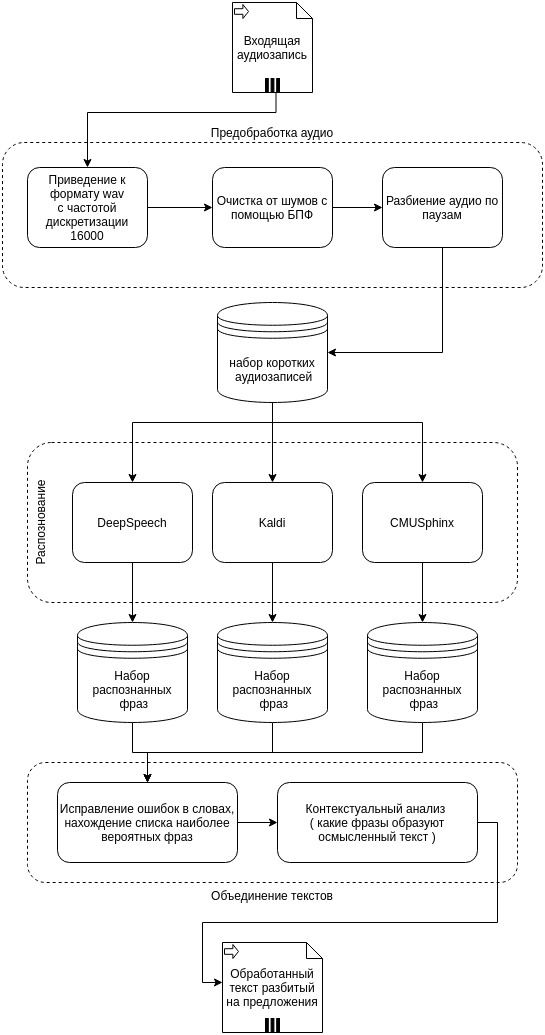
\includegraphics[width=0.4\textwidth]{./Diagram1.jpg}
\caption{Cтруктурная схема предлагаемого подхода}
\label{fig:Panel}
\end{figure}

На вход программной системы передается аудиозапись, после прохождения нескольких этапов на выходе пользователь системы получает наиболее вероятное предложение.

Первый этап, предобработка аудио. Аудиозапись приводится к заданному формату с конкретной частотой дискретизации. Затем производится очистка от шумов, например с помощью быстрого преобразования Фурье (далее БПФ). Очищенная от шумов аудиозапись разбивается на более мелкие по паузам, тем самым решается несколько проблем: во-первых, мы заранее знаем где были паузы - т.е. законченные мысли и можем это использовать при выдаче конечного результата, во-вторых, мы частично избежим проблемы смешения дикторов.

Второй этап, распознавание аудио. Полученные аудиозаписи помещаются в базу данных и маркируются как относящиеся к одному тексту. Каждая аудиозапись отправляется параллельно во все системы ASR, на выходе которых мы получаем варианты распознанной фразы. После обработки всех аудиозаписей и получения наборов распознанных фраз можно приступать к анализу текстов.

Третий этап, коррекция ошибок. Сначала мы исправляем ошибки в каждой фразе - сравнивая её с вариантами от других ASR, и составляем наиболее полное предложение. Затем в этом предложении проводится обработка последовательностей, разделенных пробелами - мы определяем является ли последовательность словом, если нет, то какие варианты слов из алфавита могут ей соответствовать. Если последовательность невозможно распознать она маркируется спецсимволом MASK.

Четвертый этап, коррекция ошибок на основе контекста. На данном этапе с помощью ручного или автоматического анализа контекста выявляется, составляют ли полученные фразы осмысленный текст. Автоматический анализ контекста предлагается производить с помощью BERT.

\subsection{Алгоритм}
Предложенный метод призван уменьшить количество ошибок и как следствие повысить качество распознавания речи. Сделать это предлагается за счет уменьшения пространства всех возможных фраз, путем использования нескольких распознающих систем и получения нескольких возможных вариантов фраз, из которых и будет производится дальнейший выбор.

Полученные фразы должны быть сопоставлены, выявление наиболее вероятных вариантов фраз происходит по следующему алгоритму (описан для трех систем).

Проверяем не состоит ли фраза из одного слова. Удаляем все пробельные символы и определяем является ли получившийся результат словом с заданным редакционным расстоянием. Если да, то обработку можно считать завершенной.

Все три варианта фразы сортируются по следующим параметрам:

\begin{itemize}
\item совпадения количества пробельных символов у нескольких фраз, это свидетельствует о правильном определении границ слов;
\item совпадения длины строки;
\item по количеству точно распознанных слов (сколько слов из фразы есть в словаре);
\item по приоритету ASR, если по какой-то причине мы доверяем одной из ASR больше.
\end{itemize}

После сортировки принимаем первую фразу за истинную. Выравниваем фразы, по совпадающим словам, заменяя пробелы вокруг совпавших слов на спецсимволы. Таким образом мы получаем границы, правильно распознанных участков.

Промежутки, находящиеся внутри спецсимволов, сравниваем по описанному выше алгоритму, не совпавшие промежутки обозначаем как не распознанные. Если ни в одном промежутке из группы нет хотя бы одного корректного слова, помечаем этот диапазон как не распознанный.

Таким образом, получаем лучшую из возможных комбинацию результатов, в которой не распознанные участки помечены спецсимволом MASK. Если предложение не удалось распознать полностью, то фраза анализируется с помощью BERT - анализатора контекста от компании Google.

\subsection{Особенности очистки шумов}
Одной из задач, которую необходимо было решить в рамках данной работы, является задача предобработки звука и удаления шумов. Нам необходимо это сделать не только для уменьшения вероятности ошибки, но и для большей однородности записей.

Есть два основных способа решения этой проблемы: модели на основе рекуррентных нейронных сетей, и различные алгоритмы спектрального анализа.
В работе был произведен сравнительный анализ двух инструментов, реализующих эти подходы: RNNoise и ffmpeg.

В рамка проекта ffmpeg разработан фильтр afftdn, предназначенный для очистки аудио от шума. В основе этого фильтра лежит алгоритм БПФ.

RNNoise — это свободный инструмент, основанный на рекуррентной нейронной сети с типом ячеек GRU. Модель RNNoise обученная на различных видах шумов, пытается анализировать аудиозапись и вычленять различные виды шума.

При практическом использовании оказалось, что фильтр afftdn справляется с задачей лучше RNNoise, и работает быстрее, поэтому для очистки шумов был выбран именно он.

\subsection{Реализация подхода}

Для реализации предложенного подхода разработана программная система, отвечающая следующим требованиям:

\begin{enumerate}
\item возможность встраивания новых процедур для обработки аудиозаписи;
\item возможность параллельного распознавания аудиозаписей с помощью ASR, следовательно необходима возможность одновременного использования одного аудио файла;
\item удобство использования и замены разных ASR использующих разные библиотеки;
\item предоставление кроссплатформенного интерфейса для работы с системой.
\end{enumerate}

Для обеспечения перечисленных требований используется ансамбль докер контейнеров, задачи которым устанавливаются через REST-API сервис,
который выступает интерфейсом для внешних пользователей и выполняет функцию брокера задач используя очередь задач.

REST-API сервис реализует архитектуру приложения ``Клиент-Сервер``, тем самым обеспечивает кроссплатформенность системы.
Использование REST-сервиса предоставляет широкие возможности для клиентских приложений. Клиентское приложение может быть написано под практически любую операционную систему, под практически любую платформу (включая мобильную), и практически на любом языке программирования.
Вместо аутентификации пользователя REST-API сервис реализует простой способ защиты данных пользователей.
При загрузке файла клиент получает уникальный ключ, полученный на основе переданной аудиозаписи, вычисленный с использованием хеш-функции.
Результат распознавания предоставляется в ответ на получение этого ключа.
Для предотвращения перехвата ключа, связь между клиентом и сервером реализована через протокол HTTPS\@.

Для того чтобы повысить отклик программной системы каждый из перечисленных сервисов должен иметь возможность обрабатывать аудиозаписи независимо.
Это сложно реализовать при обработке всей аудиозаписи целиком, поэтому решено разбивать аудиозапись на меньшие отрезки ориентируясь на паузы в речи.
По умолчанию, разбиение осуществляется на группы, в которых встречается 100 пауз по 2 секунды. Эти два параметра (длина интервала паузы и количество пауз) настраивается в системе для гибкого конфигурирования и получения наилучшего качества распознавания.
Чтобы сервисы имели возможность одновременно работать с одним и тем же участком аудиофайла каждый участок загружается в сервис хранения файлов откуда любой другой сервис может его получить.
Разбиение позволило не только использовать независимость сервисов, но и снизило время ожидания пользователем первого предложения.
Независимость работы всех компонентов позволила использовать все ASR-системы одновременно, тем самым обеспечив параллельность системы на этапе распознавания аудиозаписи.

В качестве конкретных инструментов для реализации были выбраны:

\begin{enumerate}
\item язык разработки - Python3.6;
\item очередь задач - Redis;
\item сервис конвертации и очистки от шума - ffmpeg;
\item сервис диаризации - pyAudioAnalysis;
\item сервис хранения файлов - Scality S3;
\item сервисы ASR - Kaldi, DeepSpeech, CMUSphinx.
\end{enumerate}


\subsection{Результаты}
Результаты работы программной системы были оценены по показателям WER и SF для тестовой аудиозаписи, содержащей зашумленную русскую речь.
Тестовая запись обладает следующими характеристиками:

\begin{itemize}
\item 15 минут записи - 1400 слов;
\item 17Мб;
\item 128 Kbit/sec;
\item 3\% шума.
\end{itemize}

Замеренные показатели сравнивались со средним значением трех ASR систем, лежащих в основе программной системы.
На проверочном наборе данных предложенная система показала ухудшение по показателю SF в среднем на 27\%.
Другими словами, программная система работает медленнее, что объясняется большим количеством компонентов.
По показателю WER программная система показала результаты лучше на 7\%, снизив количество ошибок за счет контекстного анализа.

\section{Заключение}
В работе приведен обзор методов преобразования аудиозаписей в текст. Проведен сравнительный анализ существующих реализаций для рассмотренных методов, на основе которого сделан вывод что интегральные системы пока что немного уступают в точности распознавания гибридным СММ/ИНС моделям.

Представлен интеграционный подход, который комбинирует различные ASR с системами улучшения аудио и обработкой текста.

Приведены детали реализации и проведен анализ результатов по двум метрикам качества, который показывает выигрыш используемого метода над существующими подходами.


\begin{thebibliography}{00}
\bibitem{b1} Using the Doc2Vec Algorithm to Detect Semantically Similar Jira Issues in the Process of Resolving Customer Requests  Kovalev, A., Voinov, N., Nikiforov, I. 2020 Studies in Computational Intelligence
\bibitem{b2} Федеральный закон от 27.07.2006 n 152-фз (ред. от 31.12.2017) "О персональных данных"
\bibitem{b3} Балакшин Павел Валерьевич. Алгоритмические и программные средства распознавания речи на основе скрытых марковских моделей для телефонных служб поддержки клиентов: диссертация кандидата технических наук: 05.13.11 / Балакшин Павел Валерьевич;[Место защиты: Федеральное государственное автономное образовательное учреждение высшего образования «Санкт-Петербургский национальный исследовательский университет информационных технологий, механики и оптики»].- Санкт-Петербург, 2015.- 127 с.
\bibitem{b4} Марковников, Н. М., и И. С. Кипяткова. Аналитический обзор интегральных систем распознавания речи. Труды СПИИРАН, т. 3, вып. 58, June 2018, сс. 77-10, doi:10.15622/sp.58.4.
\bibitem{b5} Карпов Алексей Анатольевич, Кипяткова Ирина Сергеевна. "Методология оценивания работы систем автоматического распознавания речи" Известия высших учебных заведений. Приборостроение, vol. 55, no. 11, 2012, pp. 38-43.
\bibitem{b6} Прытков В.А. "Функция расстояния между строками на основе кусочно-постоянной модели" Доклады Белорусского государственного университета информатики и радиоэлектроники, no. 4 (74), 2013, pp. 22-28.
\bibitem{b7} Comparing Speech Recognition Systems (Microsoft API, Google API And CMU Sphinx) Këpuska V, Bohouta G
\bibitem{b8} Zaity B., Wannous H., Shaheen Z., Chernoruckiy I., Drobintsev P., Pak V. "A hybrid convolutional and recurrent network approach for conversational AI in spoken language understanding." (2019).
\bibitem{b9} Makovkin K.A. [Hybrid models – Hidden Markov Models/Multilayer perceptron and their application in speech recognition systems. Servey]. Rechevye tehnologii – Speech Technology. 2012. vol. 3. pp. 58–83. (In Russ.).
\bibitem{b10} Markovnikov N.M., Kipyatkova I., Karpov A., Filchenkov A. Deep neural networks in Russian speech recognition. Proceedings of 2017 Artificial Intelligence and Natural Language Conference. 2017. pp. 54–67
\bibitem{b11} Levenshtein V.I. Binary codes capable of correcting deletions, insertions, and reversals. Soviet physics. Doklady. 1996. vol. 10. pp. 707–710.
\bibitem{b12} Yen-Lu Chow and Richard Schwartz. 1989. The N-Best algorithm: an efficient procedure for finding top N sentence hypotheses. In Proceedings of the workshop on Speech and Natural Language (HLT ’89). Association for Computational Linguistics, USA, 199–202. DOI:https://doi.org/10.3115/1075434.1075467
\bibitem{b13} Ronzhin A.L., Karpov A.A., Li I.V. Rechevoj i mnogomodal'nyj interfejsy [Speech and multimodal interfaces]. М.: Nauka. 2006. 173 p. (In Russ.).
\bibitem{b14} Kipyatkova I., Karpov A. DNN-Based Acoustic Modeling for Russian Speech Recognition Using Kaldi. International Conference on Speech and Computer. 2016. pp. 246–253.
\bibitem{b15} LeCun Y., Bengio Y. Convolutional networks for images, speech, and time series. The handbook of brain theory and neural networks. 1995. vol. 3361. no. 10. pp. 1995.
\bibitem{b16} Романенко А.Н., Матвеев Ю.Н., and Минкер В.. "Перенос знаний в задаче автоматического распознавания русской речи в телефонных переговорах" Научно-технический вестник информационных технологий, механики и оптики, vol. 18, no. 2, 2018, pp. 236-242.
\bibitem{b17} Povey D. et al. The Kaldi speech recognition toolkit». IEEE 2011 workshop on automatic speech recognition and understanding. IEEE Signal Processing Society. 2011. 4 p.
\end{thebibliography}
\vspace{12pt}

\end{document}

